\documentclass[12pt]{ociamthesis}  % default square logo 
%\documentclass[12pt,beltcrest]{ociamthesis} % use old belt crest logo
%\documentclass[12pt,shieldcrest]{ociamthesis} % use older shield crest logo

%load any additional packages
\usepackage{listings}
\usepackage{amssymb}
\usepackage{multirow}
\usepackage{caption}
\usepackage{titlesec}
\usepackage{charter}
\usepackage{subfiles}
\usepackage{etoolbox} %halaman I-1
%\patchcmd{\addcontentsline}
 % {\thepage}
  %{\thechapter-\thepage}
  %{}
  %{}

\makeatletter
\@addtoreset{subsubsection}{chapter}
\makeatother
\renewcommand{\thepage}{\thechapter-\number\numexpr\arabic{page}\relax}
\patchcmd{\cleardoublepage}{\ifodd}{\unless\ifodd}{}{}
\preto\chapter{\cleardoublepage}
\AtBeginDocument{\setcounter{page}{1}}





\makeatletter					%
\renewcommand*\@pnumwidth{3em}	% ratain halaman daftar isi
\makeatother					%

\title{\large CHAPTER 3\\[1ex]     %your thesis title,
        }   %note \\[1ex] is a line break in the title
        

\author{Diajukan untuk memenuhi kelulusan matakuliah Pemrograman II 
pada Program Studi DIV Teknik Informatika\\[5ex]
O l e h : \\
[1ex] Echa Dwiifanka   \\ 
\textbf{1.18.4.022}\\
		 [5ex] } 
		 
\college{}  %your college

%\renewcommand{\submitt edtext}{change the default text here if needed}
\degree{POLITEKNIK POS INDONESIA}    %the degree
\degreedate{\textbf{BANDUNG\\2019}}  

%end the preamble and start the document
\begin{document}

%this baselineskip gives sufficient line spacing for an examiner to easily
%markup the thesis with comments
\baselineskip=18pt plus1pt

%set the number of sectioning levels that get number and appear in the contents
\setcounter{secnumdepth}{3}
\setcounter{tocdepth}{3}


\maketitle          % create a title page from the preamble info

   
\chapter*{Teori}

\begin{enumerate}
	\item CSV(Comma Separated Value) adalah format data yang digunakan para pengguna untuk menginputkan data kedalam database secara sederhana.

	\begin{itemize}
	\item Fungsi file CSV adalah format basis data sederhana yang di setiap record dipisahkan dengan tanda koma dan titik koma.
	\end{itemize}
	
	\begin{figure} [h]
	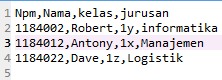
\includegraphics[width=5cm]{poto/1.png}
	\centering
	\end{figure}		
	
	
	
	
	\item Aplikasi yang dapat membuat file CSV adalah Notepad,Worpad,Microsoft Excel,dll
	
	\item Cara membuat file CSV:
	\begin{itemize}
	\item Buka Ms.Excell
	\end{itemize}
	\begin{itemize}
	\item Membuat data di Ms.Excel
	\end{itemize}
	\begin{itemize}
	\item Lalu pada saat menyimpan pilih "save as" dan jenis file nya diganti csv
	\end{itemize}
	\begin{itemize}
	\item Dan file CSV telah dibuat
	\end{itemize}

	\item library csv adalah format yang sudah digunakan selama bertahun-tahun dengan cara standar di RFC 4180. Perbedaan halus terdapat di beberapa aplikasi.
	
	
	\item library Pandas adalah alat analisis data dan struktur unruk bahasa pemrograman Python.  Panda digunakan dengan mudah untuk mengelola data salah satu fiturnya adalah Dataframe. Dataframe dapat digunakan untuk membaca sebuah file dan menjadikannya table.


	\item Fungsi yang terdapat pada library CSV:\\
	\begin{itemize}
	\item Reade, Fungsi Reader diguunakan untuk membaca  isi file
	\end{itemize}
	\begin{itemize}
	\item Dict Reader, Fungsi Dict Reader digunakan untuk membaca isi file yang terdapat di dictionary
	\end{itemize}
	\begin{itemize}
	\item Write, Fungsi Write ini digunakan untuk menulis file
	\end{itemize}
	\begin{itemize}
	\item Dict Write, Fungsi Dict Write digunakan untuk menulis file yang ada di dictionary
	\end{itemize}
	
	\item Fungsi yang terdapat di libarary pandas
	\begin{itemize}
	\item to\_csv, untuk menulis file yang type nya CSV
	\end{itemize}
	\begin{itemize}
	\item read\_csv, untuk membaca file type CSV
	\end{itemize}
	
	
\end{enumerate}





\end{document}

